
%% Template for Master thesis
%% ===========================
%%
%% You need at least KomaScript v3.0.0,
%% e.g. available in Texlive 2009
\documentclass[12pt, a4paper, twoside]{book}
\usepackage[a4paper,left=3cm,right=2cm,top=2.5cm,bottom=2.5cm,bindingoffset=5mm]{geometry}
\usepackage{setspace}

% used pagages
\usepackage[utf8]{inputenc}
\usepackage[T1]{fontenc}
\usepackage[english]{babel}

\usepackage{amsmath}
\usepackage{amssymb}
\usepackage{amsfonts}
\usepackage{slashed}

\usepackage{graphicx}
\graphicspath{{./plots/}}
\usepackage{subcaption}

\usepackage{feynmp-auto}

\usepackage{cite}
\bibliographystyle{abbrv}
\usepackage{hyperref}

\usepackage{appendix}

% german date setup
\usepackage[ngerman]{datetime}
\newdateformat{myformat}{\THEDAY{ten }\monthnamengerman[\THEMONTH], \THEYEAR}

% colours
\usepackage{color}
\definecolor{darkblue}{rgb}{0.0,0.0,0.4}
\definecolor{darkgreen}{rgb}{0.0,0.4,0.0}

% links
\hypersetup{
    colorlinks,
    linkcolor=black,
    citecolor=darkgreen,
    urlcolor=darkblue
}

\newcommand{\brac}[1] {\!\left(#1\right)}

\begin{document}
\unitlength = 1mm
\pagestyle{empty}


%% this will generate title pages similar to the template provided
%% by the Department of Physics and Astronomy Heidelberg
%%
%% More information:
%% http://www.physik.uni-heidelberg.de/aktuelles/studium/
%% (PDF link: ...studium/download/145/Vorlage_Diplomarbeit_Formular.pdf)

%% Titleintro
\thispagestyle{empty}
\begin{center}
  \renewcommand{\baselinestretch}{2.00}
  \Large\sffamily
  Department of Physics and Astronomy\\
  \large University of Heidelberg
  \par\vfill\normalfont
  Master thesis\\
  in Physics\\
  submitted by\\
  David Conway Lafferty\\
  born in Glasgow\\
  1994
\end{center}
\cleardoublepage

%% Titlepage
\thispagestyle{empty}
\begin{center}
  \renewcommand{\baselinestretch}{2.00}
  \Large\bfseries\sffamily
    (Title)\\
    (of)\\
    (Master thesis)
  \par
  \vfill
  \large\normalfont
  This Master thesis has been carried out by David Conway Lafferty\\
  at the\\
  Institute of Theoretical Physics\\
  under the supervision of\\
  Prof. Dr. Jan M. Pawlowski\\
  \& \\
  Dr. Alexander K. Rothkopf\\
  %% additionally insert second supervisor here if carrying out an
  %% external diploma thesis. Reduce vspace in L. 44 accordingly.
\end{center}\par
\vspace{5\baselineskip}

% reset baselinestretch
\renewcommand{\baselinestretch}{1.00}\normalsize
\cleardoublepage

\cleardoublepage

\pagenumbering{roman}
\pagestyle{plain}

%% Abstract page
%% =============
%%
%% Content of abstract pages has been put into seperate pages to simplify
%% word counting. Use e.g. the unix command
%%   wc abstract-ger.tex
%% or
%%   wc abstract-eng.tex
%% to get the number of words contained in these files.
\thispagestyle{empty}
\begin{center}
  \begin{minipage}[c][0.48\textheight][b]{0.9\textwidth}
    \small
    \textbf{
      (Titel der Masterarbeit - deutsch):
    }\par
    \vspace{\baselineskip}
    %% Latex markup und Zitate funktionieren auch hier
(Abstract in Deutsch, max. 200 Worte. Beispiel: \cite{loremIpsum})

Lorem ipsum dolor sit amet, consectetur adipisici elit, sed eiusmod tempor
incidunt ut labore et dolore magna aliqua. Ut enim ad minim veniam, quis
nostrud exercitation ullamco laboris nisi ut aliquid ex ea commodi consequat.
Quis aute iure reprehenderit in voluptate velit esse cillum dolore eu fugiat
nulla pariatur. Excepteur sint obcaecat cupiditat non proident, sunt in culpa
qui officia deserunt mollit anim id est laborum.

Duis autem vel eum iriure dolor in hendrerit in vulputate velit esse molestie
consequat, vel illum dolore eu feugiat nulla facilisis at vero eros et
accumsan et iusto odio dignissim qui blandit praesent luptatum zzril delenit
augue duis dolore te feugait nulla facilisi. Lorem ipsum dolor sit amet,
consectetuer adipiscing elit, sed diam nonummy nibh euismod tincidunt ut
laoreet dolore magna aliquam erat volutpat.

Ut wisi enim ad minim veniam, quis nostrud exerci tation ullamcorper suscipit
lobortis nisl ut aliquip ex ea commodo consequat. Duis autem vel eum iriure
dolor in hendrerit in vulputate velit esse molestie consequat, vel illum dolore
eu feugiat nulla facilisis at vero eros et accumsan et iusto odio dignissim qui
blandit praesent luptatum zzril delenit augue duis dolore te feugait nulla
facilisi.
  \end{minipage}\par
  \vfill
  \begin{minipage}[c][0.48\textheight][b]{0.9\textwidth}
    \small
    \textbf{
      (Title of Master thesis - english):
    }\par
    \vspace{\baselineskip}
    %% Latex markup and citations may be used here
Lorem ipsum dolor sit amet, consectetur adipisici elit, sed eiusmod tempor
incidunt ut labore et dolore magna aliqua. Ut enim ad minim veniam, quis
nostrud exercitation ullamco laboris nisi ut aliquid ex ea commodi consequat.
Quis aute iure reprehenderit in voluptate velit esse cillum dolore eu fugiat
nulla pariatur. Excepteur sint obcaecat cupiditat non proident, sunt in culpa
qui officia deserunt mollit anim id est laborum.

Duis autem vel eum iriure dolor in hendrerit in vulputate velit esse molestie
consequat, vel illum dolore eu feugiat nulla facilisis at vero eros et
accumsan et iusto odio dignissim qui blandit praesent luptatum zzril delenit
augue duis dolore te feugait nulla facilisi. Lorem ipsum dolor sit amet,
consectetuer adipiscing elit, sed diam nonummy nibh euismod tincidunt ut
laoreet dolore magna aliquam erat volutpat.

Ut wisi enim ad minim veniam, quis nostrud exerci tation ullamcorper suscipit
lobortis nisl ut aliquip ex ea commodo consequat. Duis autem vel eum iriure
dolor in hendrerit in vulputate velit esse molestie consequat, vel illum dolore
eu feugiat nulla facilisis at vero eros et accumsan et iusto odio dignissim qui
blandit praesent luptatum zzril delenit augue duis dolore te feugait nulla
facilisi.
  \end{minipage}
\end{center}


\cleardoublepage

\cleardoublepage

\tableofcontents

\cleardoublepage

\pagenumbering{arabic}
\chapter{Introduction}
\onehalfspacing 
The strong interaction is the strongest of the four fundamental forces of nature. It is described by quantum chromodynamics (QCD), a quantum field theory exhibiting many peculiar properties. The first, known as asymptotic freedom, is that the underlying interaction strength of QCD decreases as the relevant energy scale increases. Another, which is still not completely understood, is colour confinement -- the phenomenon that the fundamental degrees of freedom of QCD, quarks and gluons, do not exist as isolated objects and instead form bound states known as hadrons. Hadrons make up most of the matter we experience in our everyday lives, and thus colour confinement is observed ubiquitously at the rather mundane energy scales that are naturally present on Earth. However, a more exotic state of matter is theorised to exist at extremely high temperatures or densities -- the Quark Gluon Plasma (QGP). In the QGP, quarks and gluons are considered as being asymptotically free and no longer confined to within the bounds of a hadron. More generally speaking, the QGP is expected to be one of many regions in the entire phase space of strongly interacting matter. A schematic phase diagram is shown in Fig.~\ref{fig:QCDphasediag}, where one can see for example the location of neutron stars at high density and low temperature. Indeed, the QGP itself is believed to have existed in the early moments of our universe, and thus understanding its properties will form a crucial part of answering some of the deepest questions of human thought.  

The monumental experimental effort aimed at detecting and quantifying the QGP has culminated today in the relativistic heavy-ion colliders such at those at BNL, CERN, and GSI. The complexity of such experiments has necessitated the development of new techniques both in experiment and theory, in order to firstly map the measured experimental data to QGP properties (a highly non-trivial process) and then to understand how these macroscopic properties emerge from the underlying microscopic theory of QCD. With regards to the former, one refers to various ``probes'' that may indicate the presence of QGP formation. This thesis revolves around one such probe, namely heavy quarkonium.

The bound states of a heavy quark and anti-quark of the same flavour are known generically as quarkonia. Since the seminal work of Matsui and Statz [REF], the interest in quarkonium as a probe of the QGP has grown into a considerable subfield in the realm of heavy ion collisions. From an experimental perspective, an intricate and not yet fully understood structure has emerged in the production and decay of these mesons throughout the collision process. From the theory side, the development of new effective field theories [REF] has allowed quantitative predictions to be made from ever more rigorous formalisms. One such formalism, known as pNRQCD, relies on separating the typical scales present in the system, so that the dynamics of the bound state are governed by an effective potential in a non-relativistic Schro{\"o}dinger equation [REF]. In this way, the complexities of the full quantum field theory are reduced to a much more tractable quantum mechanical problem.

This thesis presents a new prescription for parametrising the static heavy-quark potential in a background of hot and deconfined charge carriers, such as the QGP. By generalising the Gauss law of classical electromagnetism and combining this with a field-theoretic in-medium permittivity, the resulting in-medium complex potential admits an analytical solution. This can then be used to calculate spectral functions, and give realistic phenomenological predictions. The outline of this thesis is as follows: in Chapter \ref{sec:theory_ov}, we give a short summary of some theoretical aspects of QCD, as well as an introduction into quarkonium phenomenology both in vacuum and in the context of heavy ion collisions. Chapter \ref{sec:med_pot} provides a detailed derivation of the in-medium potential and shows that this parametrisation is able to faithfully reproduce lattice data by utilising only one fitting parameter, the inverse screening length. Chapter \ref{sec:app_HIC} outlines the procedure with which phenomenologically relevant quantities such as the melting temperatures, decay widths, and electromagnetic decay ratios can be calculated. The main results of this thesis are also given here, and a comparison is made with recent experimental results. A summary and outlook is given in Chapter \ref{sec:conc}. Appendix A contains a short introduction to thermal field theory and in particular the notion of a spectral function. Appendix B gives a more formal derivation of the Debye mass at one-loop order via Euclidean thermal field theory and finally, Appendix C shows how the structure of the in-medium permittivity arises from the Schwinger-Keldysh formalism. 

\begin{figure}
	\centering
	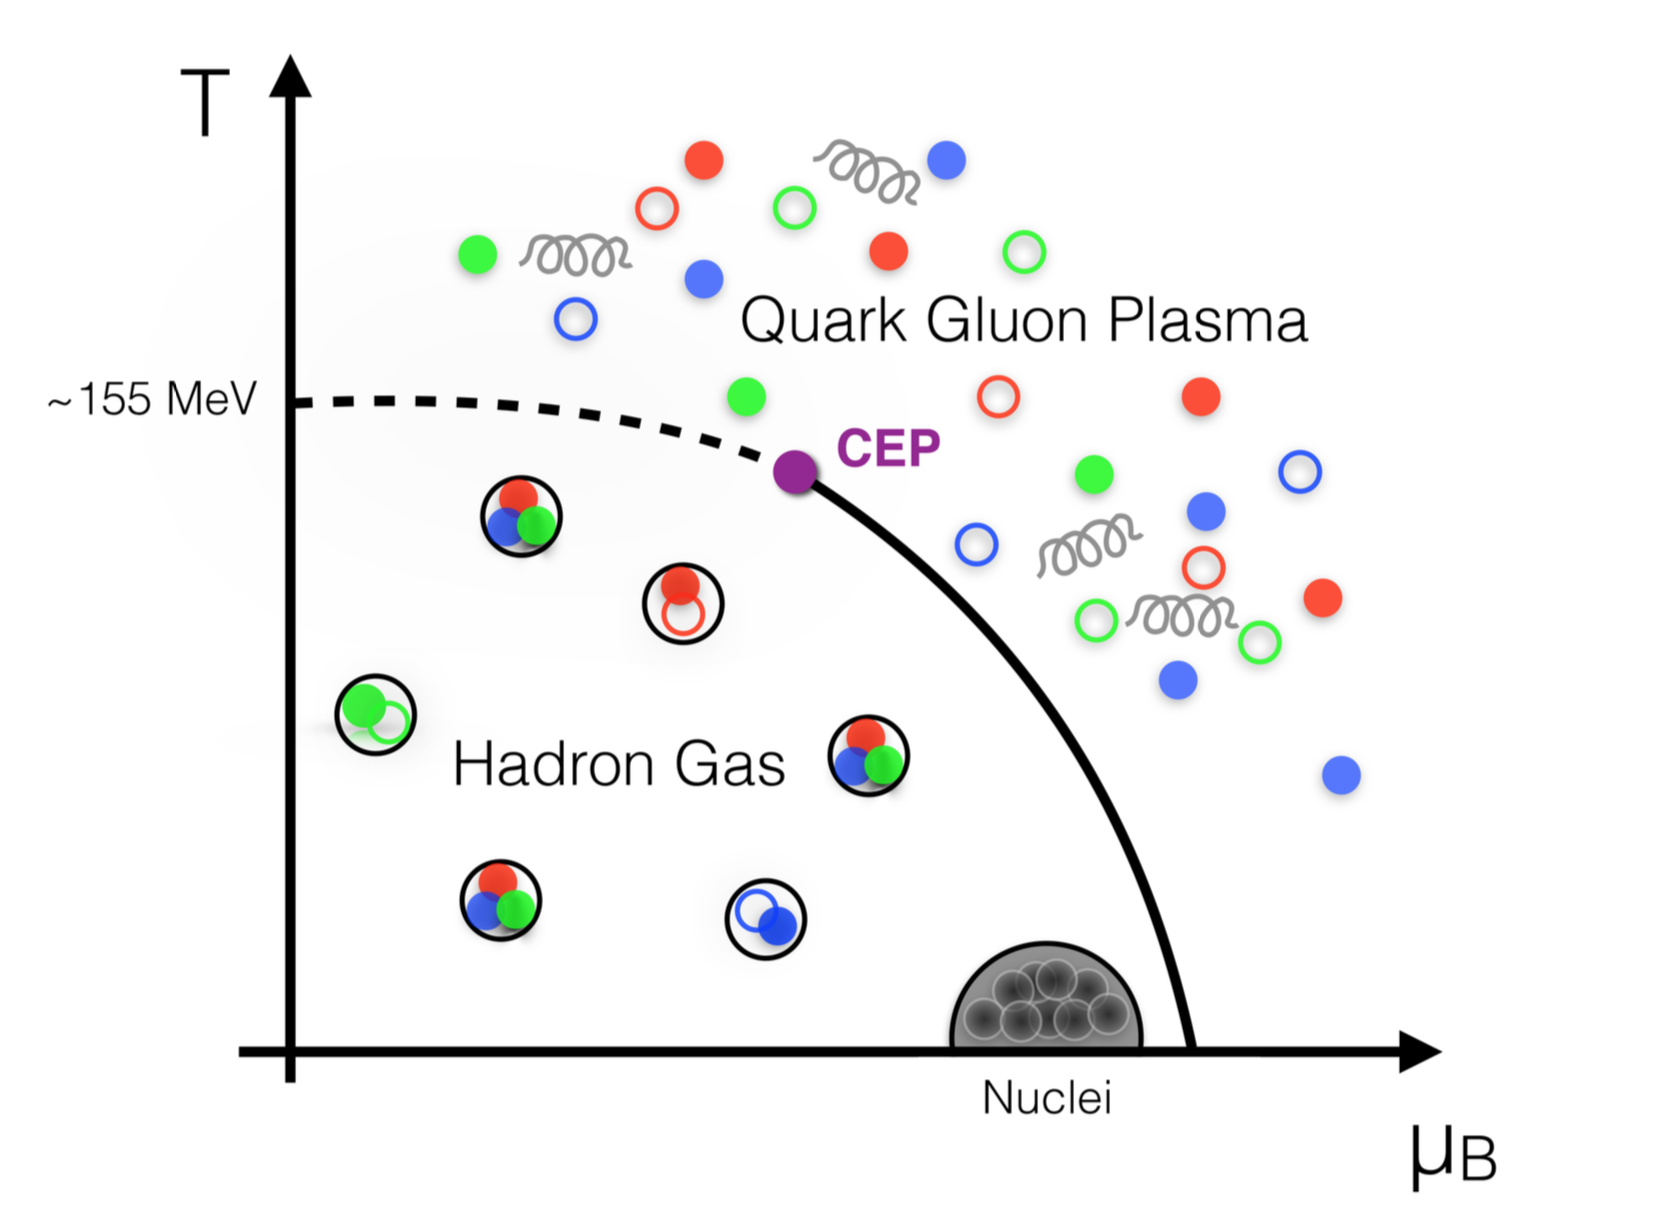
\includegraphics[width=0.9\textwidth]{QCDphase}
	\caption{A qualitative QCD phase diagram.}\label{fig:QCDphasediag}
\end{figure}

\chapter{Theory overview}
\label{sec:theory_ov}
\onehalfspacing
In this Chapter, we provide the theoretical foundations of various topics that will be important throughout the rest of this thesis. We start with an introduction into quantum chromodynamics, by constructing the Lagrangian and looking at the fundamental interactions. Some more insight will be given on the phenomena of confinement and asymptotic freedom, before a brief discussion of QCD thermodynamics and the phase diagram. The presentation here will mainly follow [REF] where the reader can consult for more details. We then give an overview of vacuum heavy quarkonium physics by outlining some of the techniques used to discern for example the numerous quantum states in the heavy quark anti-quark system. Finally, we introduce some important concepts in heavy ion collisions, with an emphasis on heavy quarkonium phenomenology. 
\section{Aspects of QCD}
In the 1970s, Murray Gell-Mann and George Zweig independently proposed a model to explain the observed spectrum of strongly interacting particles that contained the idea of \emph{quarks} as elementary particles of fractional charge that exist within hadrons. While explaining and predicting some aspects very well, the quark model contained notable flaws. Namely, the lack of observation of free particles with fractional charge, and the existence of some states apparently in violation of the well-established exclusion principle that quarks, as fermions, must obey. The resolution of the first problem was the introduction of a new, additional quantum number termed \emph{colour}. Each quark would carry one of three possible colour charges -- red, green, or blue, -- the symmetry properties of which mitigated the existence of the problematic states. The second problem was solved by the discovery that non-Abelian gauge theories exhibit asymptotic freedom [REF], which allowed the theory of strong interactions to be brought into its final form. Namely, quantum chromodynamics, a non-Abelian gauge theory with colour symmetry group \(SU\brac{3}\), coupled to quarks acting under the fundamental representation. As is often the case in science, we have had the luxury of summarising decades of previous generations' work in a mere few sentences, glossing over the murky and often enlightening details. For a more detailed historical account of the development of QCD, a nice read is [REF].  

\subsection{QCD Lagrangian}
As a quantum field theory, the fundamental object of QCD is its Lagrangian density (often denoted simply as the Lagrangian), \(\mathcal{L}_{QCD}\), which we now proceed to construct based on the guiding properties outlined in the previous paragraph. The quarks and anti-quarks are described respectively by the Dirac spinor fields 
\begin{equation}
\psi_{\alpha,i,f}\brac{x}, \quad\quad \bar{\psi}_{\alpha,i,f}\brac{x},
\end{equation} 
where \(\alpha\) is the spinor index representing the underlying Poincar\'e invariance, \(i=1,2,3\) is the colour index, \(f=1\ldots N_{F}\) labels the flavour quantum number (\(f=\) up, down, strange, charm, bottom, top), and \(x\) is the position 4-vector. The free quark Lagrangian is then
\begin{equation}
\label{eq:quarklag}
\mathcal{L}_{quark}=\sum_{f}\sum_{i}\bar{\psi}_{\alpha,i,f}\brac{x}\brac{i\brac{\gamma^{\mu}\partial_{\mu}}_{\alpha\beta}-M_{\alpha\beta}}\psi_{\beta,i,f}\brac{x},
\end{equation}
where \(M_{\alpha\beta}=\delta_{\alpha\beta}m_f\) is the quark mass matrix. At this point we impose local gauge invariance as necessitated by the non-Abelian nature of the theory. That is, we require the Lagrangian to remain invariant under the following transformation (neglecting indices):
\begin{equation}
\psi '\brac{x}=U\brac{x}\psi\brac{x},\quad\quad\bar{\psi}'\brac{x}=\bar{\psi}\brac{x}U^\dagger\brac{x},
\end{equation}
where the transformation matrix 
\begin{equation}
U\brac{x}=e^{i\epsilon\left(x\right)}=e^{i\sum\epsilon_a\brac{x} t_a}
\end{equation}
acts on the colour indices. The group parameters are \(\varepsilon_a\brac{x}\) and the group generators, which are the Gell-Mann matrices matrices for \(SU\brac{3}\), are denoted \(t_a\). For a comprehensive overview of the role of group theory in particles physics, the reader can consult [REF]. One can easily verify that the mass term in Eq.~\eqref{eq:quarklag} remains invariant under a gauge transformation, however the spacetime derivative in the kinetic term does not. The resolution is to promote the partial derivative to the covariant derivative 
\begin{equation}
D_\mu=\partial_\mu-igA_\mu
\end{equation}
where the gauge field \(A^\mu\brac{x}=\sum_a A^\mu_a\brac{x}t_a\) is associated to the force-mediating bosons (gluons) and \(g\) is the coupling strength. Local gauge invariance now requires the gluon field to transform as 
\begin{equation}
A_\mu '=UAU^\dagger + \frac{i}{g}U\brac{\partial_\mu U^\dagger}.
\end{equation}
Finally, a kinetic term describing the gluon dynamics is required. The gluon field strength tensor is defined as the commutator of two covariant derivatives:
\begin{equation}
\label{eq:gluonfst}
F_{\mu\nu}\brac{x}=\frac{i}{g}\left[D_\mu,D_\nu \right]=\partial_\mu A\nu - \partial_\nu A_\mu-ig\left[A_\mu,A_\nu\right].
\end{equation}
To see how this structure arises naturally from geometric considerations, the reader can consult [REF] for an excellent treatment. Eq.~\eqref{eq:gluonfst} transforms as \(F_{\mu\nu}'=UF_{\mu\nu}U^\dagger\), from which we can deduce that a gluon mass term \(\sim m_g A_\mu A^\mu\) would break gauge invariance and hence cant not appear in the Lagrangian -- gluons are massless. Contracting two field strength tensors does not lead to a gauge invariant object and one must additionally take the trace in colour space,
\begin{equation}
\mathrm{Tr}\{F'^{\mu\nu}F'_{\mu\nu}\}=\mathrm{Tr}\{F^{\mu\nu}F_{\mu\nu}\}=F^a_{\mu\nu}F_{b}^{\mu\nu}\mathrm{Tr}\{t_at^b\}\sim F^a_{\mu\nu}F_{a}^{\mu\nu}.
\end{equation} 
With this, we are able to write down the QCD Lagrangian in all of its glory. Holding the sum over flavour and colour indices in Eq.~\eqref{eq:quarklag} as implicit, using Feynman slash notation and neglecting the Dirac indices, the Lagrangian takes on the following aesthetically pleasing form:
\begin{equation}
\label{eq:qcdlagr}
\mathcal{L}_{QCD}=\bar{\psi}\brac{x}\brac{i\slashed{D}-M}\psi\brac{x}-\frac{1}{4}F^a_{\mu\nu}F_a^{\mu\nu}.
\end{equation}
The above equation is the most fundamental realisation of the strong nuclear force. It is often deemed beautiful that the huge and rich variety of emergent physical phenomena associated with the strong force can be attributed in principle to a single equation. 

\subsection{Asymptotic freedom}
We now proceed to examine the interactions that arise from Eq.~\eqref{eq:qcdlagr} at the level of quarks and gluons, and investigate some of their consequences. The first term in Eq.~\eqref{eq:qcdlagr} contains a quadratic expression in the fermion field \(\psi\) which describes the propagation of a non-interacting particle. It also couples the fermion field to the gauge field \(A\) through the \(A\) term in the covariant derivative, giving rise to a three-point interaction vertex. Without explicitly expanding the second term, one can easily observe that it will give rise to expressions \(\sim\!A^2, \sim\!A^3\) and \(\sim\!A^4\). The expression quadratic in the gauge fields will eventually describe the propagation of free gluons, although it should be noted here that one must first quantise the theory in a self-consistent way by using the Faddeev-Popov method which is rather non-trivial [REF]. The expressions \(\sim\!A^3\) and \(\sim\!A^4\) describe gluonic self-interactions. These are unique to QCD as compared to for example the Abelian theory of quantum electrodynamics (QED), and play a vital role in the plethora of highly non-trivial QCD dynamics. The diagrammatic representations of each expression above is given in Fig.~\ref{fig:qcdtree}. 
\begin{figure}
    \centering
    \begin{subfigure}[b]{0.3\textwidth}
    	\begin{fmffile}{QCDfermion}
    		\begin{fmfgraph}(40,25)
    		\fmfleft{i1}
    		\fmfright{o1}
    		\fmf{vanilla}{i1,o1}
    		\end{fmfgraph}
    	\end{fmffile}
        \caption{Free quark propagator}
    \end{subfigure}
    \begin{subfigure}[b]{0.3\textwidth}
    	\begin{fmffile}{QCDgluon}
    		\begin{fmfgraph}(40,25)
    		\fmfleft{i1}
    		\fmfright{o1}
    		\fmf{gluon}{i1,o1}
    		\end{fmfgraph}
    	\end{fmffile}
        \caption{Free gluon propagator}
    \end{subfigure}
    \vspace*{10mm}

    \begin{subfigure}[b]{0.3\textwidth}
    	\begin{fmffile}{QCDfermglu}
    		\begin{fmfgraph}(40,25)
    		\fmfleft{i1,i2}
    		\fmfright{o1}
    		\fmf{vanilla}{i1,v1}
    		\fmf{vanilla}{i2,v1}
    		\fmf{gluon}{o1,v1}
    		\fmfdot{v1}
    		\end{fmfgraph}
    	\end{fmffile}
        \caption{Quark-gluon vertex}
    \end{subfigure}
    \begin{subfigure}[b]{0.3\textwidth}
    	\begin{fmffile}{QCDglu3}
    		\begin{fmfgraph}(40,25)
    		\fmfleft{i1,i2}
    		\fmfright{o1}
    		\fmf{gluon}{i1,v1}
    		\fmf{gluon}{i2,v1}
    		\fmf{gluon}{o1,v1}
    		\fmfdot{v1}
    		\end{fmfgraph}
    	\end{fmffile}
    	\vspace*{5mm}
        \caption{Cubic gluon vertex}
    \end{subfigure}    
    \begin{subfigure}[b]{0.3\textwidth}
    	\begin{fmffile}{QCDglu4}
    	\begin{fmfgraph}(40,25)
    		\fmfleft{i1,i2}
    		\fmfright{o1,o2}
    		\fmf{gluon}{i1,v1}
    		\fmf{gluon}{i2,v1}
    		\fmf{gluon}{o1,v1}
    		\fmf{gluon}{o2,v1} 	
    		\fmfdot{v1}
    		\end{fmfgraph}
    	\end{fmffile}
    \vspace*{5mm}
    \caption{Quartic gluon vertex}
    \end{subfigure}
    \vspace*{4mm}
    \caption{Tree-level QCD diagrams.}
   	\label{fig:qcdtree}
\end{figure}

Before being able to quantitatively understand asymptotic freedom, we must first introduce \emph{renormalisation} and the concept of a running coupling. Although it is recognised today that quantum field theory (QFT) is the only consistent framework that can emerge from the union of quantum mechanics and special relativity [REF:weinberg1], this was by no means obvious in its historical development. In the early days, quantum field theoretic tools could be used to describe some physical processes with good accuracy, however its usefulness was certainly not ubiquitous. The theory also exhibited some worrying features -- most notably, the emergence of unphysical infinities when calculating scattering amplitudes beyond leading order. QFT was considered so sick that even its most ardent practitioners acknowledged the need for something of an overhaul, with many physicists advocating employing somewhat different formalisms to describe the most fundamental interactions [REF].

The remedy eventually came by way of renormalisation. The modern picture is as follows: the expressions describing fundamental processes often contain divergent integral expressions, which are nonetheless able to be quantified and isolated by the process of \emph{regularisation}. Then, the free parameters such as the masses and coupling constant in a Lagrangian like Eq.~\eqref{eq:qcdlagr} are interpreted as `bare' and unphysical. They must be split into a physical part and a corresponding unphysical `counter-term' that will cancel the infinities present in the theory. In this way, the divergences are swept under the proverbial rug, leaving the physical parameters that must be measured in experiment. This was seen by some as a cheap trick when first introduced, however with the advent of Kenneth Wilson's renormalisation group originating from statistical physics, it is today valued as an indispensable tool in describing the physical world. In the Wilsonian viewpoint the subtraction of infinity can be seen as an admission of our ignorance, in the sense that we introduce a cut-off scale at large momenta or small distances, beyond which the theory is not expected to hold. The renormalisation group is a fascinating tool that permeates many areas of theoretical physics today, with powerful accompanying ideas and extensions such as universality. The interested reader can refer to [REFS], with QFT applications being given in [REF].

One consequence of renormalisation is that the physical parameters inherit a scale dependence. Much like the way in which the spring constant in Newton's second law depends on the make-up of the spring and can only be measured in mechanical experiments, the physical masses and coupling constants of a renormalised quantum field theory will depend on the momentum (or equivalently, distance) scale probed by a particular collider experiment. In the case of a given coupling constant, this phenomenon is known generically as the running of the coupling. One can calculate (via the renormalisation procedure outlined above) to a given order how the coupling constant will change as the momentum scale is changed. This is usually expressed via the beta function
\begin{equation}
\label{eq:betafunc}
\beta\brac{g\brac{\mu}}=\frac{\partial g\brac{\mu}}{\partial \mathrm{log}\brac{\mu}},
\end{equation}
where \(g\) is the relevant coupling constant evaluated at momentum scale \(\mu\). For QCD the relevant diagrams at one-loop order are shown in Fig.~\ref{fig:QCDbeta_oneloop} and the result is [REF]
\begin{equation}
\label{eq:betaQCD_oneloop}
\beta_{QCD}\brac{g}\lvert_{\mathrm{1-loop}}=-b\frac{g^3}{16\pi^2}+\mathcal{O}\brac{g^5}
\end{equation}
where \(b=11-\frac{2}{3}N_F\) and \(N_F\) is the number of flavours. The minus sign in Eq.~\eqref{eq:betaQCD_oneloop} is of tremendous importance. It implies that for \(N_F\leq 16\) the QCD coupling constant decreases as the energy or momentum scale increases. Defining the more commonly used \(\alpha_s=\frac{g^2}{4\pi}\), the beta-function can be integrated to give
\begin{equation}
\label{eq:gQCD_oneloop}

\end{equation}

\section{Quarkonium in vacuum}
\label{sec:quark_vav}
\onehalfspacing
\chapter{The in-medium potential}
\label{sec:med_pot}
\onehalfspacing
\chapter{Application to Heavy Ion Collisions}
\label{sec:app_HIC}
\onehalfspacing
\chapter{Conclusion}
\label{sec:conc}
\onehalfspacing

\begin{appendices}
\chapter{Debye mass derivation}
\chapter{Schwinger-Keldysh formalism}
\end{appendices}

\bibliography{references}

\chapter*{Acknowledgements}


\cleardoublepage
\setlength{\parindent}{0em}

Erkl\"{a}rung:\par
\vspace{3\baselineskip}
Ich versichere, dass ich diese Arbeit selbstst\"{a}ndig verfasst habe und keine
anderen als die angegebenen Quellen und Hilfsmittel benutzt habe.\par
\vspace{5\baselineskip}
Heidelberg, den (Datum)\hspace{3cm}\dotfill


\end{document}
